\subsection{Estrutura do trabalho} \label{subsec:estrutura}

 Este documento está estruturado em~\ref{sec:conclusoes} capítulos, divididos da seguinte forma:
 

    
    \begin{figure}[H]
    	\centering
    	\caption{Estrutura da dissertação}
    	\label{fig:estrutura}
    	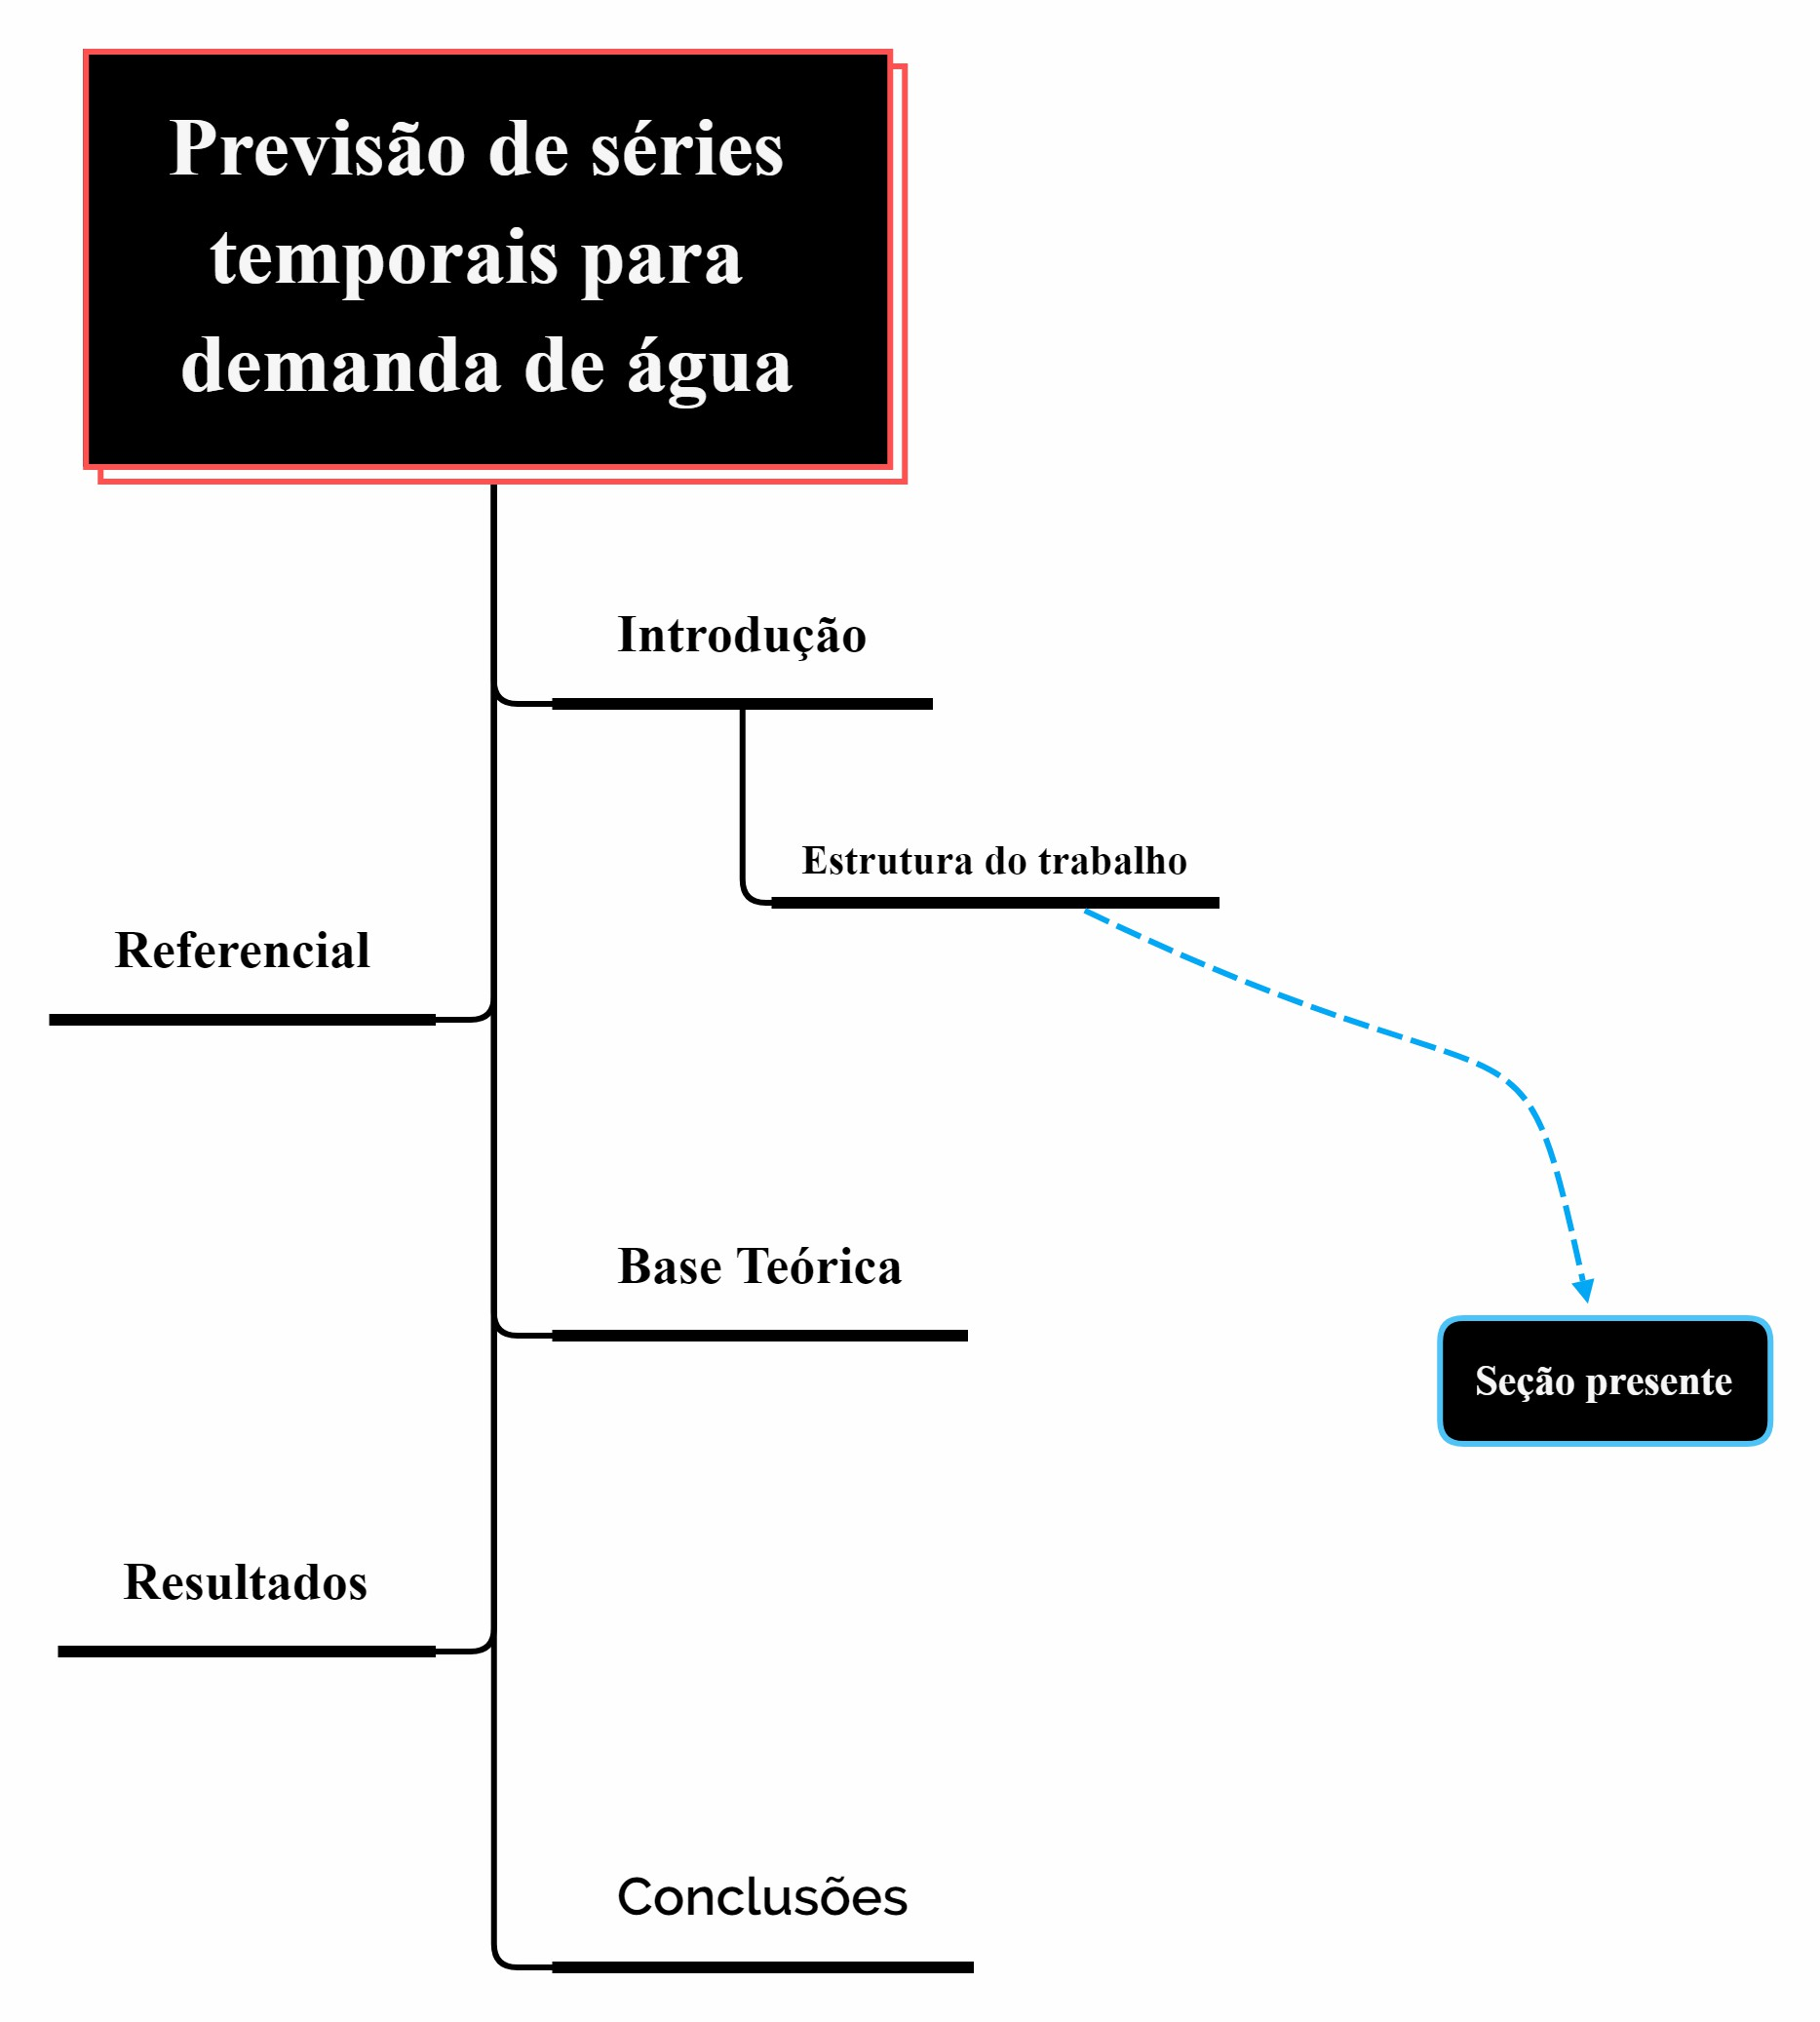
\includegraphics[width=0.7\linewidth]{Introducao/Figuras/Estrutura}
    	
    	Fonte: Elaboração própria 
    \end{figure}
O capítulo~\ref{sec:int} apresenta a introdução do trabalho, contendo a contextualização, a motivação, o objetivo geral, os objetivos específicos, a metodologia utilizada, a justificativa da pesquisa, as contribuições, as publicações e a organização do trabalho.
O capítulo~\ref{sec:refteo} apresenta a descrição do problema, revisão teórica do trabalho, fazendo uma visão geral dos principais pesquisadores sobre as questões abordadas na pesquisa.
O capítulo~\ref{sec:base} apresenta os modelos que serão trabalhados nos dados coletados.
O capítulo~\ref{sec:result} apresenta os resultados da pesquisa, assim como uma análise dos resultados gerados.
O capítulo~\ref{sec:conclusoes}, finalmente, apresenta as considerações finais da pesquisa e algumas propostas para pesquisas futuras.
